\documentclass[12pt]{article}
\usepackage{listings}
\usepackage{graphicx}
\usepackage{amsmath}
\begin{document}
\begin{titlepage}
   \begin{center}
       \vspace*{1cm}
       \large
       \textbf{Project 2: Feature Detection and Matching}
       \normalsize

       \vspace{0.5cm}

       Author: Gabriel Hofer

       \vspace{0.5cm}

       CSC-414 Introduction to Computer Vision

       \vspace{0.5cm}

       Instructor: Dr. Hoover

       \vspace{0.5cm}

        March 31, 2020

       \vfill

       Computer Science and Engineering\\
       South Dakota School of Mines and Technology\\
   \end{center}
\end{titlepage}
%------------------------------------------------------------------------------------
\newpage

% can write this in latex - just an example
% 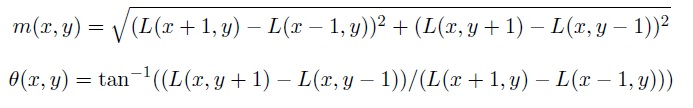
\includegraphics[scale=0.5]{sift-orientation-eqns.jpg}


\small
\textbf{Introduction}\\ 



\textbf{Step 1}\\ 
Harris Corner Detection



Harris Matrix



magnitude and orientation
\[
    m(x,y) = \sqrt{(L(x+1,y)-L(x-1,y))^2+(L(x,y+1)-L(x,y-1))^2}
\]
\[
    \theta (x,y) = \arctan{(L(x,y+1)-L(x,y-1))/(L(x+1,y)-L(x-1,y))}
\]
How to create bins:

save images of showFeature -- and then put them here in the writeup

\textbf{Step 2: Descriptors}\\

\textbf{Step 3: Feature Matching}\\



\end{document}


